\documentclass[a4paper]{article}

\usepackage[english]{babel}
\usepackage[utf8x]{inputenc}
\usepackage{amsmath}
\usepackage{graphicx}
\usepackage[colorinlistoftodos]{todonotes}

\title{CMSC 471 Artificial Intelligence\\
	Project 2 Optimization Problems}
\author{Siqi Lin\\
	Prof.Maksym Morawski}

\begin{document}
\maketitle

\section{Introduction}

The purpose of this paper is to demonstrate the performance of three different local search algorithms, hill climbing, hill climbing with random restarts and simulated annealing. While all three of the optimization strategy aim to find the minimum value, simulated annealing has a superior performance than the other two searches.

\section{Local Searches}

\subsection{Hill Climbing}
Hill climbing is the brute-force local search among the three local searches. Given an arbitrary starting point, it will simply loop continuously in the direction of an uphill move and it will terminate the loop when a maximum point is found among its neighbors. Many might perceive the hill climbing technique as a greedy local search because it always obtains the best value among one's neighbor without considering the entire graph as a whole.Therefore, hill climbing can reach obstacles in the following situations, 1) a local max/min is found, 2) a ridge is observed, 3) a plateau is encountered.

\subsection{Hill Climbing with Random Restarts}
The Hill climbing with random restarts strategy performs a series of hill climbing operations from randomly generated points. While the regular hill climbing search is not nearly complete, the hill climbing with random restarts has a relatively higher level of completeness by performing hill climbing numerous times.  

\subsection{Simulated Annealing}
Simulated annealing is an approximating search strategy to find the maximum value. By incorporating a control parameter, T, which is the temperature function, the probability of a good move can be estimated. The simulated annealing strategy only accepts a new change when the calculated probability indicates a good move. Below is the equation to calculate the probability of good move versus a bad move.
$$P(move_{A-B}) \approx \mathrm{e}^{\frac{f(B)-f(A)}{T}}$$

\section{Comparison of Local Searches}
\subsection{Performance}
The purpose of the project is to implement hill climbing, hill climbing with random restarts and simulated annealing and find the minimize the given function below.
$$z = \frac{\sin(x^2 + 3y^2) }{0.1+r^2}+ (x^2+5y^2) + \exp(1-r^2)$$
      $$ r = \sqrt{x^2 + y^2}$$
After implementing and executing all three searches using the same parameters, such as the range for x and y values, the objective function, and step size, simulated annealing turns out to have the most optimal solution among the three searches. Because the three-dimensional function has various local minimum values throughout the graph, using hill climbing can always lead to a bottleneck when a local minimum value is found. Hill climbing search would consider the local minimum to be the global minimum because the neighboring points of the local minimum all have higher values than the local minimum. On the other hand, hill climbing with random restarts is much efficient then the hill climbing strategy. With random starting points at each restart, it reduce the possibility of excessively exploring around a initial starting point. By generating a new starting point, more space can be explored and the chance of finding an optimal solution is higher. While the CPU time for hill climbing with random restart can be costly, it's more efficient than hill climbing in the sense that more space of the graph gets explored. In addition, the simulated annealing search also outperform the regular hill climbing search. Because simulated annealing includes a control parameter, T, the temperature function, to calculate a probability of a good move, it can utilize the calculated probability value to estimate and decide if a move can be made. Similar to the hill climbing with random restart search, simulate annealing also has a random search feature to ensure more space are explored. With the temperature function, as temperature decreases, the global minimum will shortly be found. However, there's also an issue with simulated annealing. Because the temperature is critical to the entire algorithm, the implementation and design of the temperature function can be cumbersome. Despite the After implementing and executing all three searches using the same parameters, such as the range for x and y values, the objective function, and step size, simulated annealing turns out to have the most optimal solution among the three searches. Because the three-dimensional function has various local minimum values throughout the graph, using hill climbing can always lead to a bottleneck when a local minimum value is found. Hill climbing search would consider the local minimum to be the global minimum because the neighboring points of the local minimum all have higher values than the local minimum. On the other hand, hill climbing with random restarts is much efficient then the hill climbing strategy. With random starting points at each restart, it reduce the possibility of excessively exploring around a initial starting point. By generating a new starting point, more space can be explored and the chance of finding an optimal solution is higher. While the CPU time for hill climbing with random restart can be costly, it's more efficient than hill climbing in the sense that more space of the graph gets explored. In addition, the simulated annealing search also outperform the regular hill climbing search. Because simulated annealing includes a control parameter, T, the temperature function, to calculate a probability of a good move, it can utilize the calculated probability value to estimate and decide if a move can be made. Similar to the hill climbing with random restart search, simulate annealing also has a random search feature to ensure more space are explored. With the temperature function, as temperature decreases, the global minimum will shortly be found. However, there's also an issue with simulated annealing. Because the temperature is critical to the entire algorithm, the implementation and design of the temperature function can be cumbersome. Despite the importance of the temperature function, most of the time, the simulated annealing search would outperform both the hill climbing search and the hill climbing with random restart search.  
In terms of CPU time, hill climbing with random restarts would have higher CPU time than hill climbing given the number of restarts. Simulated annealing also has a dependent variable when it comes to CPU time, the starting temperature can alter the execution time of the search. With the initial temperature being high, the executing time would take longer and vice verse for low initial temperature. 
\section{Generated Output}
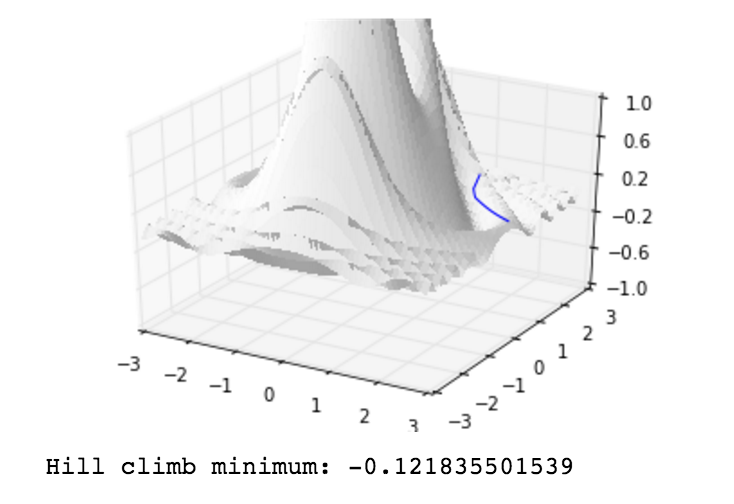
\includegraphics[scale=0.5]{hill_climb}
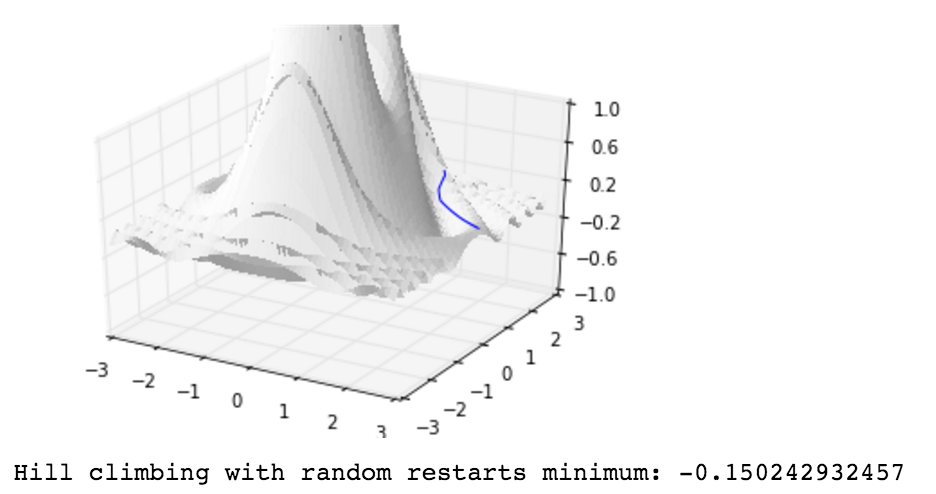
\includegraphics[scale=0.5]{hill_climb_random_restart}
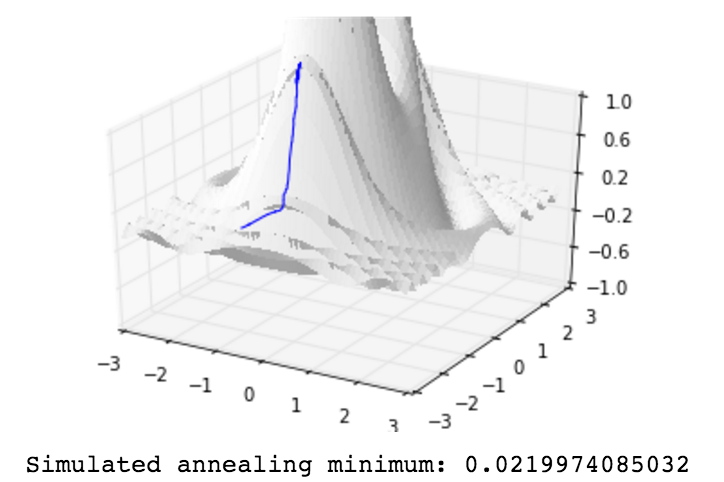
\includegraphics[scale=0.5]{simulated_annealing}
\section{Reference}
\begin{enumerate}
  \item $https://en.wikipedia.org/wiki/Hill_climbing$
  \item $http://matplotlib.org/users/pyplot_tutorial.html$
  \item $https://en.wikibooks.org/wiki/LaTeX/Mathematics$
  \item $https://confluence.cornell.edu/display/CS472/Simulated+Annealing,+Random+Restarts$
  \item https://www.sharelatex.com/learn/
\end{enumerate}

\end{document}